\chapter{Application: SASI Toy Problem}
\label{chap:application}

As mentioned at the beginning of Chapter~\ref{chap:introduction}, the simple toy model of FS~\cite{Foglizzo2009,Sato2009} was chosen as a useful initial application of our well-balanced method to the SASI. The salient details from those papers  are reproduced here. Following the notation of FS, we will denote quantities in the supersonic region before the shock with a subscript `1', in the interior region between the shock and potential step with `in', and in the outflow region past the step with `out'.

A schematic view of the problem domain can be seen in Fig.~\ref{fig:Sato1}, showing how the overall scenario is split into two sub-problems for simulation. The entire test case consists of an supersonic inflow deccelerated at a stationary shock front, followed shortly after by a potential step which further slows the now subsonic flow. This provides a very simplistic analogue to study the mechanisms at play during the inflow, decceleration, and accretion of matter in a collapsing star before supernova.

\begin {figure}
\centering
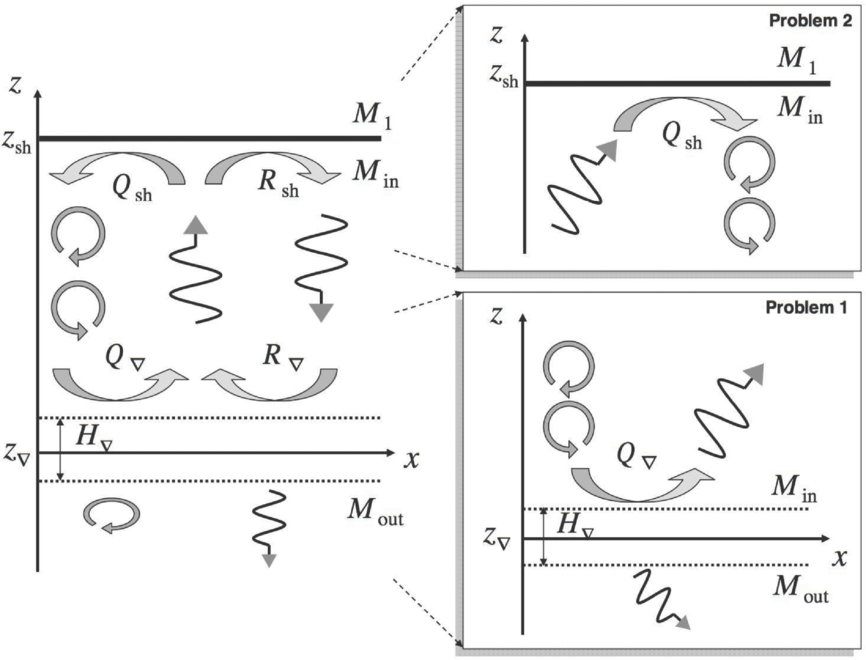
\includegraphics[width=13cm]{figures/Sato1}
\caption {A short caption.}
\label{fig:Sato1}
\end{figure}

For ease of simulation, the potential step and stationary shock are computed separately as sub-problems 1 and 2 respectively. This separation greatly simplifies the introduciton of specific advective and acoustic pertubations to appropriate locations in the interior of the domain, making it much easier to see the interactions of these disturbances at the boundaries (the shock and potential step) between the various flow regions.


\section{Problem Set-up}
\label{sec:TP_set_up}

We have a shock defined by the Rankine-Hugoniot conditions...
\begin{align}
\mathcal{M}_\textrm{in}&=\sqrt{\frac{2+(\gamma-1)\mathcal{M}_1^2}{2\gamma\mathcal{M}_1^2-\gamma+1}},\\
\frac{v_1}{v_\textrm{in}}&=\frac{(\gamma+1)\mathcal{M}_1^2}{2+(\gamma-1)\mathcal{M}_1^2},\\
\frac{\rho_1}{\rho_\textrm{in}}&=\frac{v_\textrm{in}}{v_1},
\end{align}

A hyperbolic tangent function is used to provide a smooth step-like external potential field, with the exact function given by
\begin{equation}
\phi(y)=\frac{\Delta\phi}{2}\left[\tanh\left(\frac{y-y_{\nabla}}{H_{\nabla}/2}\right)+1\right],
\end{equation}
where the step size $\Delta\phi$ is set based on the ratio of the sound speeds $c_{\textrm{in}}/c_{\textrm{out}}$ in the constant regions surrounding the step.

\begin{equation}
\Delta\Phi=\left(\frac{\mathcal{M}_\textrm{out}^2}{2}+\frac{1}{\gamma-1}\right)c_\textrm{out}^2-\left(\frac{\mathcal{M}_\textrm{in}^2}{2}+\frac{1}{\gamma-1}\right)c_\textrm{in}^2
\end{equation}

\begin{equation}
\tau_\textrm{aac}\equiv\frac{1}{1-\mathcal{M}_\textrm{in}}\frac{H}{|v_\textrm{in}|}
\end{equation}

\subsection{Sub-Problem 1: Potential Step}
\label{subsec:sub_problem_1}

Perturbations are given by...
\begin{equation}
\delta S\equiv\epsilon_S\cos\left(-\omega_0t+k_xx+k_yy\right)
\end{equation}

\begin{equation}
\frac{\delta \rho}{\rho_\textrm{in}}\equiv\exp\left(-\frac{\gamma-1}{\gamma}\delta S\right)-1
\end{equation}

\begin{equation}
\delta v_x\equiv\frac{k_x\omega_0c_\textrm{in}^2}{\omega_0^2+k_x^2v_\textrm{in}^2}\frac{\delta S}{\gamma} \quad \textrm{and} \quad \delta v_y\equiv\frac{k_x^2v_\textrm{in}c_\textrm{in}^2}{\omega_0^2+k_x^2v_\textrm{in}^2}\frac{\delta S}{\gamma}
\end{equation}

\begin{equation}
\delta w_y=-\frac{k_xc_\textrm{in}^2}{v_\textrm{in}}\frac{\epsilon_S}{\gamma}\sin\left(-\omega_0t+k_xx+k_yy\right)
\end{equation}

\subsection{Sub-Problem 2: Standing Shock}
\label{subsec:sub_problem_2}

Description of the standing shock

\begin{align}
\frac{\delta\rho}{\rho_\textrm{in}}&\equiv\frac{1+\mu\mathcal{M}_\textrm{in}}{1-\mathcal{M}_\textrm{in}^2}\epsilon_\rho\cos\left(-\omega_0t+k_xx+k_y^-y\right) \\
\frac{\delta p}{p_\textrm{in}}&\equiv\left(1+\frac{\delta\rho}{\rho_\textrm{in}}\right)^\gamma-1 \\
\delta v_x&\equiv\frac{k_xc_\textrm{in}^2}{\omega_0}\epsilon_\rho\cos\left(-\omega_0t+k_xx+k_y^-y\right) \\
\delta v_y&\equiv\frac{\mu+\mathcal{M}_\textrm{in}}{1-\mathcal{M}_\textrm{in}^2}c_\textrm{in}\epsilon_\rho\cos\left(-\omega_0t+k_xx+k_y^-y\right) \\
\delta T
\end{align}

\begin{equation}
\mu\equiv\sqrt{1-\frac{k_x^2c_\textrm{in}^2}{\omega_0^2}\left(1-\mathcal{M}_\textrm{in}^2\right)}
\end{equation}

\begin{equation}
k_y^\pm=\frac{\omega}{c_\textrm{in}}\frac{\mathcal{M}_\textrm{in}\mp\mu}{1-\mathcal{M}_\textrm{in}^2}
\end{equation}